%% Diagram illustrating how a communication channel might be mapped onto a
%% simplified SpiNNaker machine.
\documentclass[tikz]{standalone}
\usetikzlibrary{arrows.meta, decorations.pathreplacing, positioning}
\usepackage{times}

\begin{document}
  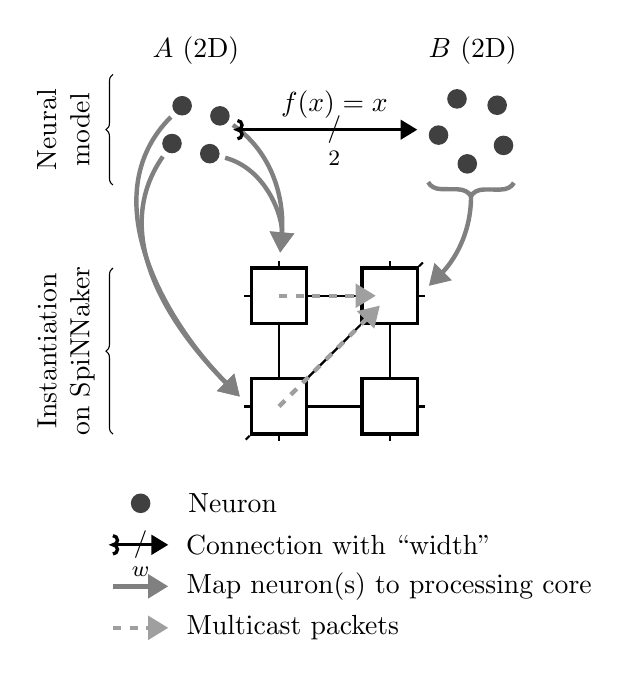
\begin{tikzpicture}[
      neuron/.style = {fill=black!75!white, text width=5pt, text height=5pt,
                       inner sep=0pt, circle},
      projection/.style = {very thick, ->, shorten <= 15pt, shorten >= 20pt,
                           arrows={Hooks[reversed]-Triangle[]}},
      map base/.style = {ultra thick, draw=black!50!white},
      map/.style = {map base, shorten >= 5pt, shorten <= 2pt,
                    arrows={-Triangle[]}},
      map brace/.style = {map base, decoration={brace, amplitude=5pt}, decorate},
      core/.style = {draw, very thick, inner sep=0pt, text width=2em,
                     text height=2em},
      link/.style = {thick},
      packet stream/.style = {gray!75!white, ultra thick, dashed, shorten >= 5pt, arrows={-Triangle[]}},
    ]
    %% Draw the neural populations (4 neurons to 5 neurons)
    \begin{scope}
      \node [above] (a) at (0, 20pt) {$A$ (2D)};
      \foreach \n in {1,...,4}{%
        \node (A\n) [neuron] at (\n * 90 + 30:10pt) {};
      }
    \end{scope}

    \begin{scope}[xshift=10em]
      \node [above] (b) at (0, 20pt) {$B$ (2D)};
      \foreach \n in {1,...,5}{%
        \node (B\n) [neuron] at (\n * 72 + 45:12.5pt) {};
      }
    \end{scope}

    %% Draw a simplified representation of the SpiNNaker architecture
    \begin{scope}[xshift=3em, yshift=-10em]
      \foreach \x in {0,1} {%
        \foreach \y in {0,1} {%
          \node (core\x\y) [core] at (\x*4em, \y*4em) {};
        }
      }

      \foreach \n in {0,1}{%
        \draw [link] (core\n0) -- (core\n1);
        \draw [link] (core0\n) -- (core1\n);
        \draw [link] (core0\n.west) -- ++(-2pt, 0);
        \draw [link] (core1\n.east) -- ++(2pt, 0);
        \draw [link] (core\n1.north) -- ++(0, 2pt);
        \draw [link] (core\n0.south) -- ++(0, -2pt);
      }
      \draw [link] (core00) -- (core11);
      \draw [link] (core00.south west) -- ++(-1.4pt, -1.4pt);
      \draw [link] (core11.north east) -- ++(1.4pt, 1.4pt);
    \end{scope}

    %% Connect the neurons to their ``processing cores''
    \draw [map] (A1) to [in=135, out=225] (core00.west);
    \draw [map] (A2) to [in=135, out=235] (core00.west);
    \draw [map] (A3) to [in=85, out=-15] (core01.north);
    \draw [map] (A4) to [in=85, out=-35] (core01.north);
    \draw [map brace] ([yshift=-13.5pt] B4.east) -- ([yshift=-17pt] B2.west)
      node [midway, coordinate] (B) {};
    \draw [map] ([xshift=0pt, yshift=-3pt] B) to [out=-90, in=45] (core11.east);

    %% The connection between the populations
    \draw [projection]
      ([yshift=-20pt] a.south) -- ([yshift=-20pt] b.south)
      node [midway, above] {$f(x) = x$}
      node [midway, label={[yshift=5pt]below:\footnotesize 2}] {/};

    %% This connection as packet streams on SpiNNaker links
    \draw [packet stream] (core00.center) -- (core11.center);
    \draw [packet stream] (core01.center) -- (core11.center);

    %% Label the logical sections (not necessary?)
    \draw [decoration={brace}, decorate] (-3em, -2em) -- ++(0, 4em)
      node [midway, sloped, above=5pt, text width=5em, align=center]
        {Neural model};
    \draw [decoration={brace}, decorate] (-3em, -11em) -- ++(0, 6em)
      node [midway, sloped, above=3pt, text width=7em, align=center]
        {Instantiation on SpiNNaker};

    %% Add a legend
    \begin{scope}[xshift=-2em, yshift=-13.5em]
      \begin{scope}
        \node [neuron] (legend_neuron) {};
        \node [right=1em of legend_neuron] {Neuron};
      \end{scope}
      \draw [projection, shorten >= 0pt, shorten <= 0pt]
            (-1em,-1.5em) -- ++(2em, 0)
            node [midway, label={[yshift=5pt]below:\footnotesize $w$}] {/}
            node [pos=1.0, right=.25em] {Connection with ``width''};
      \draw [map, shorten >= 0pt, shorten <= 0pt]
            (-1em,-3.0em) -- ++(2em, 0)
            node [pos=1.0, right=.25em] {Map neuron(s) to processing core};
      \draw [packet stream, shorten >= 0pt, shorten <= 0pt]
            (-1em,-4.5em) -- ++(2em, 0)
            node [pos=1.0, right=.25em, black] {Multicast packets};
    \end{scope}
  \end{tikzpicture}
\end{document}
